\subsection*{Self-Supervised Learning for 3D Medical Image Analysis using
3D SimCLR and Monte Carlo Dropout}

% \subsection*{Ссылка} \url{https://arxiv.org/abs/2109.14288}
\subsubsection*{Введение} 
Self-supervised обучение проявило себя как мощный инструмент,
позволяющий конструировать значимые представления из неразмеченных
данных, что может быть использовано в задачах с малым количеством 
размеченных данных. В данной статье \cite{ann14} авторы представляют метод, 
который использует возможности SimCLR в сегментации 3D изображений.
Также показано, что дополнительное включение неопределенности 
посредством Байесовского вывода в форме метода Монте-Карло
значительно улучшает производительность в задаче сегментации.

\subsubsection*{Основная идея}
Метод состоит из трех частей: сначала производится self-supervised 
обучение энкодера, далее энкодер дообучается под необходимую 
задачу сегментации с использованием размеченных данных, а затем 
применяется метод Монте-Карло во время предсказания и вычисляется 
Dice score на тестовом множестве. \par
Если рассматривать метод более детально, то в первую очередь 
решается предварительная задача, которая обобщает SimCLR до 
трехмерных входов для исследования трехмерного пространственного контекста.
Случайным образом 3D сканы разбиваются на батчи размером \(M\), затем каждый скан 
делится на \(P\) равных неперекрывающихся 3D патча, в результате получая \(N=M*P\)
входных примеров. К входным данным применяется два случайных типа аугментации.
Архитектура модели, решающая предзадачу следующая: энкодер (3D-CNN), за ним следует 
слой нелинейной проекции (Dense layer). \par
Для решения основной задачи использовался предобученный энкодер без слоя нелинейной 
проекции. Выходы энкодера подаются на вход декодеру (U-Net), который тренируется 
уже на размеченных данных.
\subsection*{Данные}
BraTS 2018, 3D КТ сканы с опухолями поджелудочной железы (ПЖЖ).
\subsection*{Результаты}

% \begin{minipage}{1.0\linewidth}
%     \begin{center}
%         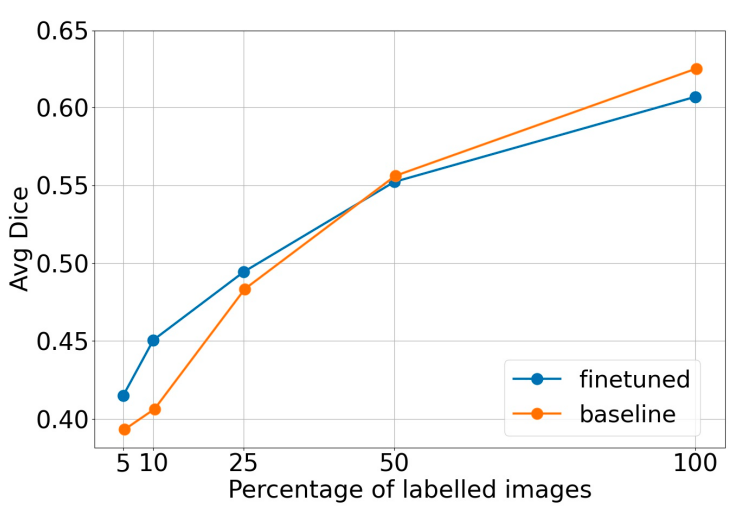
\includegraphics[scale=0.3]{ann14_res1.png} \\
%         \captionof{figure}{\scriptsize{
%             Средний Dice коэффициент после дообучения модели на 5\%,
%             10\%, 25\%, 50\%, 100\% снимков ПЖЖ. 
%             3D SimCLR модель (синий) превосходит baseline (оранжевый), когда доступно менее, чем 
%             25\% данных.
%         }}
%     \end{center}
    
% \end{minipage}
% \\
% \begin{minipage}{1.0\linewidth}
%     \begin{center}
%         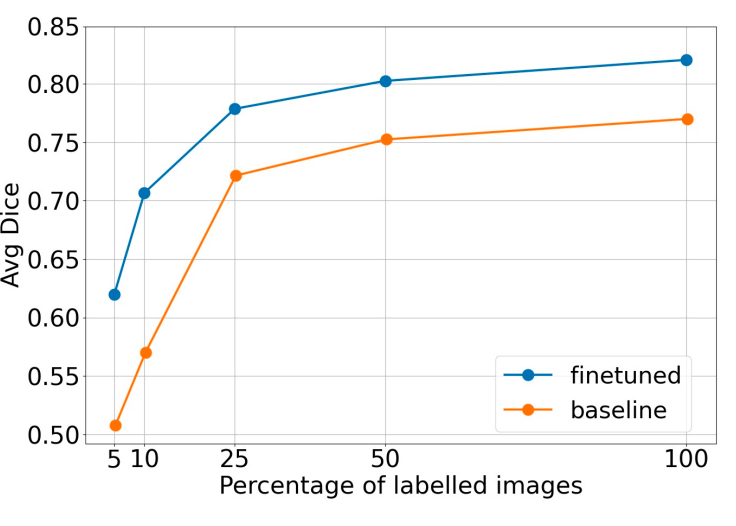
\includegraphics[scale=0.3]{ann14_res2.png} \\
%         \captionof{figure}{\scriptsize{По оси Y - средний Dice коэффициент после дообучения модели на 5\%,
%         10\%, 25\%, 50\%, 100\% тренировочного множества (BraTS).Предложенная 
%         модель - синяя линия, baseline - оранжевая.}}
%     \end{center}
    
% \end{minipage} 


\begin{minipage}{1.0\linewidth}
    \begin{center}
        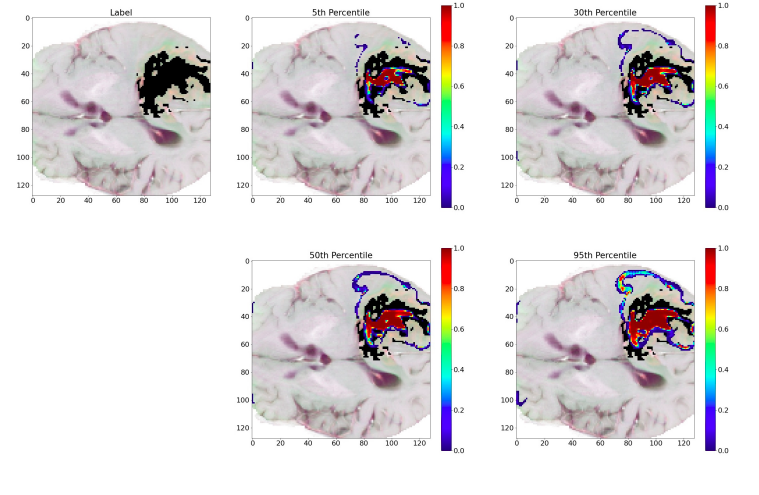
\includegraphics[scale=0.3]{ann14_mri.png} \\
        \captionof{figure}{\scriptsize{Тепловые карты различных перцентилей предсказаний классов опухоли 
        для примера из \\ датасета BraTS. Черные пиксели представляют опухоль целиком.}}
    \end{center}
    
\end{minipage}

\subsection*{Заключение}
Результаты экспериментов показывают потенциал предлагаемого метода 3D SimCLR с 
дополненной информацией из Байесовского вывода в разрезе эффективности 
обработки данных и повышения производительности. 